\documentclass[12pt]{scrartcl}
%\usepackage{refcheck} 
\usepackage{a4}   
\usepackage{amsmath}    
\usepackage{paralist}
\usepackage{amssymb} 
\usepackage{amsfonts}  
\usepackage{mathrsfs}  
\usepackage{dsfont}
\usepackage{latexsym} 
\usepackage{xcolor}
\usepackage{bbm,exscale}
\definecolor{Myblue}{rgb}{0,0,0.6}  
\usepackage[colorlinks,citecolor=Myblue,linkcolor=Myblue,urlcolor=Myblue,pdfpagemode=None]{hyperref}
\usepackage{amsthm}
\usepackage{accents}
\usepackage[square,numbers,sort&compress]{natbib} 
\usepackage[all,cmtip]{xy}
\usepackage{ifthen} 
\usepackage{bbding}
\usepackage{stmaryrd}  
\usepackage{wasysym}
\usepackage{verbatim}
\usepackage{bbding} 
\usepackage{soul}  %allow linebreak for underlined with \ul
\usepackage[yyyymmdd,hhmmss]{datetime}
\usepackage{tikz}
\usepackage{tikz-cd}
\usepackage{tikz-3dplot}
\usepackage{pgfplots}
	\pgfplotsset{width=7cm,compat=1.8}
	%%External
%	 \usetikzlibrary{external}\tikzexternalize
%	\usetikzlibrary{decorations.pathmorphing}
%	\usetikzlibrary{decorations.pathreplacing}
	\usetikzlibrary{decorations.markings}
%	\usetikzlibrary{calc}
%	\usetikzlibrary{fadings}
%	\usetikzlibrary{matrix} 
	\usetikzlibrary{patterns}
%	\usetikzlibrary{shapes.geometric}
%	\usetikzlibrary{shadows}

%\pgfplotsset{compat=1.11}            
            

\tikzset{
    string/.style={draw=#1, postaction={decorate}, decoration={markings,mark=at position .51 with {\arrow[color=#1]{>}}}},
    costring/.style={draw=#1, postaction={decorate}, decoration={markings,mark=at position .51 with {\arrow[draw=#1]{<}}}},
    ostring/.style={draw=#1, postaction={decorate}, decoration={markings,mark=at position .47 with {\arrow[draw=#1]{>}}}},
    ustring/.style={draw=#1, postaction={decorate}, decoration={markings,mark=at position .56 with {\arrow[draw=#1]{>}}}},
    oostring/.style={draw=#1, postaction={decorate}, decoration={markings,mark=at position .43 with {\arrow[draw=#1]{>}}}},
    uustring/.style={draw=#1, postaction={decorate}, decoration={markings,mark=at position .59 with {\arrow[draw=#1]{>}}}},
    directed/.style={string=blue!50!black}, 
    odirected/.style={ostring=blue!50!black}, 
    udirected/.style={ustring=blue!50!black}, 
    oodirected/.style={oostring=blue!50!black}, 
    uudirected/.style={uustring=blue!50!black},     
    redirected/.style={costring= blue!50!black},
    redirectedgreen/.style={costring= green!50!black},
    directedgreen/.style={string= green!50!black},
    redirectedlightgreen/.style={costring= green!65!black},
    directedlightgreen/.style={string= green!65!black},
}

\tikzset{-dot-/.style={decoration={
  markings,
  mark=at position 0.5 with {\fill circle (1.875pt);}},postaction={decorate}}}

\tikzset{
	Fdot/.style={circle, draw, fill, inner sep=0pt}, 
	Odot/.style={circle, draw, inner sep=0.1pt, minimum size=0.1cm}
	}

\def\nicedashedcolourscheme{\shadedraw[top color=blue!22, bottom color=blue!22, draw=gray, dashed]}
\def\nicedashedpalecolourscheme{\shadedraw[top color=blue!12, bottom color=blue!12, draw=gray, dashed]}
\def\nicehalfpalecolourscheme{\shadedraw[top color=blue!22, bottom color=blue!22, draw=white]}
\def\nicenotpalecolourscheme{\shadedraw[top color=blue!32, bottom color=blue!32, draw=white]}
\def\nicecolourscheme{\shadedraw[top color=blue!22, bottom color=blue!22, draw=blue!22]}
\def\nicepalecolourscheme{\shadedraw[top color=blue!12, bottom color=blue!12, draw=white]}
\def\nicenocolourscheme{\shadedraw[top color=gray!2, bottom color=gray!25, draw=white]}
\def\nicereallynocolourscheme{\shadedraw[top color=white!2, bottom color=white!25, draw=white]}
\def\boringcolourscheme{\draw[fill=blue!20, dashed]}

\newcommand\tikzzbox[1]
%{pic}% 
{#1}%#1

  \tolerance 1414
  \hbadness 1414
  \hfuzz 0.3pt
  \widowpenalty=10000
  \vfuzz \hfuzz
  \raggedbottom
  
\makeatletter
\newcommand{\raisemath}[1]{\mathpalette{\raisem@th{#1}}}
\newcommand{\raisem@th}[3]{\raisebox{#1}{$#2#3$}}
\makeatother

\renewcommand{\H}{\mathcal H}
\newcommand{\Ccal}{\mathcal C}
\newcommand{\boldB}{\boldsymbol{B}}
\newcommand{\A}{\mathcal{A}}
\newcommand{\orb}{\mathcal{A}}
\newcommand{\sgn}{\mathrm{sgn}}
\renewcommand{\leq}{\leqslant}
\renewcommand{\geq}{\geqslant}

\newcommand{\E}{\text{e}} 
\newcommand{\I}{\text{i}}
\newcommand{\B}{\mathcal{B}}
\newcommand{\Borb}{\B_{\mathrm{orb}}}
\newcommand{\Beq}{\B_{\mathrm{eq}}}
\newcommand{\C}{\mathds{C}}
\newcommand{\D}{\mathds{D}}
\newcommand{\Ee}{\mathds{E}}
\newcommand{\K}{\mathds{K}}
\newcommand{\M}{\mathds{M}}
\newcommand{\N}{\mathds{N}}
\newcommand{\Q}{\mathds{Q}}
\newcommand{\R}{\mathds{R}}
\newcommand{\Z}{\mathds{Z}}
\newcommand{\IP}{\mathds{P}}
\def\1{\ifmmode\mathrm{1\!l}\else\mbox{\(\mathrm{1\!l}\)}\fi}
\newcommand{\one}{\mathbbm{1}}
\newcommand{\be}{\begin{equation}}
\newcommand{\ee}{\end{equation}}
\newcommand{\bes}{\begin{equation*}}
\newcommand{\ees}{\end{equation*}}
\newcommand{\cc}[1] {\overline{#1}}
\newcommand{\inv}[0]{{-1}}

\newcommand{\inver}[0]{\times}%{\mathrm{inv}}
\newcommand{\chirel}[0]{\chi_{\mathrm{sym}}}%{\chi_{\frac{1}{2}}}
\newcommand{\Dec}[0]{\mathrm{Dec}}
\newcommand{\interior}[1]{%
  {\kern0pt#1}^{\mathrm{o}}%
}
\newcommand{\Strat}[0]{\mathrm{Strat}}
\newcommand{\Stratdef}[0]{\mathrm{Strat}^{\mathrm{def}}}


\newcommand{\sVir}{\mathsf{sVir}}
\newcommand{\MF}{\operatorname{MF}_{\operatorname{bi}}}
\newcommand{\MFW}{\operatorname{MF}_{\operatorname{bi}}(W)}
\newcommand{\MFR}{\operatorname{MF}^\text{R}_{\operatorname{bi}}}
\newcommand{\DG}{\operatorname{DG}_{\operatorname{bi}}}
\newcommand{\DGW}{\operatorname{DG}_{\text{bi}}(W)}
\newcommand{\DGR}{\operatorname{DG}^\text{R}_{\text{bi}}}
\newcommand{\id}{\text{id}}
\newcommand{\KMF}{K_{0}(\operatorname{MF}_{\text{bi}}}
\newcommand{\Ext}{\operatorname{Ext}}
\newcommand{\Hom}{\operatorname{Hom}}
\newcommand{\End}{\operatorname{End}}
\newcommand{\modu}{\operatorname{mod}}
\def\LG{\mathcal{LG}}
\def\LGgr{\mathcal{LG}^{\mathrm{gr}}}
\def\LGgrs{\mathcal{LG}'^{\mathrm{gr}}}
\def\LGgrso{\mathcal{LG}'^{\mathrm{gr}}_{\mathrm{orb}}}
\def\LGs{\mathcal{LG}'}
\def\LGsorb{\mathcal{LG}'_{\mathrm{orb}}}
\def\LGorb{\mathcal{LG}_{\mathrm{orb}}}
\def\LGeq{\mathcal{LG}_{\mathrm{eq}}}
\newcommand{\hmf}{\operatorname{hmf}}
\newcommand{\HMF}{\operatorname{HMF}}
\newcommand{\ev}{\operatorname{ev}}
\newcommand{\eval}{\operatorname{eval}}
\newcommand{\tev}{\widetilde{\operatorname{ev}}}
\newcommand{\coev}{\operatorname{coev}}
\newcommand{\tcoev}{\widetilde{\operatorname{coev}}}
\def\lra{\longrightarrow}
% \def\lra{%
% \;%
% %%%%%%%%%%%%%%%%%%%%%% 
% \tikzzbox{\begin{tikzpicture}[scale=1.0,color=black, >=stealth, color=black, baseline=-0.1cm]
% \draw[-{stealth[length=1.6mm, scale width=1.1]}, line width=0.15mm] (0,0) -- (0.7,0);
% \end{tikzpicture}}%%popende
% %%%%%%%%%%%%%%%%%%%%%% 
% \;%
% }
\def\lmt{\longmapsto}
\DeclareMathOperator{\tr}{tr}
\DeclareMathOperator{\str}{str}
\DeclareMathOperator{\Jac}{Jac}
\def\Re{R^{\operatorname{e}}}
\DeclareMathOperator{\Res}{Res}
\newcommand*{\longhookrightarrow}{\ensuremath{\lhook\joinrel\relbar\joinrel\rightarrow}}
\newcommand*{\twoheadlongrightarrow}{\ensuremath{\relbar\joinrel\twoheadrightarrow}}
\newcommand{\Ga}[1]{\Gamma_{\hspace{-2pt}#1}}
\newcommand{\HIA}{\Hom(I,A)}
\newcommand{\ZA}{Z_A(\Hom(I,A))}
\newcommand{\gZA}{\!Z_A^\gamma(\Hom(I,A))}
\newcommand{\gA}{{}_{\gamma_A}A}
\newcommand{\Aginv}{A_{\gamma_A^{-1}}}
\newcommand{\picc}{\pi^{(\text{c,c})}_A}
\newcommand{\pirr}{\pi^{\text{RR}}_A}
\newcommand{\tpirr}{{\widetilde\pi}^{\text{RR}}} 
\newcommand{\im}{\operatorname{im}}
\DeclareMathOperator*{\eq}{=}
\DeclareMathOperator*{\congscript}{\cong}
\newcommand{\specflow}{\mathcal U_{-\frac{1}{2},-\frac{1}{2}}}
\newcommand{\Hil}{\mathcal{H}}
\newcommand{\Hpcc}{\mathcal{H}'_{\text{(c,c)}}}
\newcommand{\Hprr}{\mathcal{H}'_{\text{RR}}}
\newcommand{\Hcc}{\mathcal{H}_{\text{(c,c)}}^A}
\newcommand{\Hrr}{\mathcal{H}_{\text{RR}}^A}
\newcommand{\HccnoA}{\mathcal{H}_{\text{(c,c)}}}
\newcommand{\HrrnoA}{\mathcal{H}_{\text{RR}}}
\newcommand{\Hrrbo}{\Hom_A(X,{}_{\gamma_A}X)}
\newcommand{\buboorb}{\beta_X^{\text{orb}}}
\newcommand{\bobuorb}{\beta^X_{\text{orb}}} 
\def\Cong{C_g}
\def\Centg{N_g}
\def\alphaKK{\alpha^{\{K\}}}
\def\alphagKg{\alpha_g^{K(g)}}
\newcommand{\AGC}{A_G^c}

\newcommand{\Bord}{\operatorname{Bord}}
\newcommand{\Bordor}{\operatorname{Bord}_{n}^{\mathrm{or}}}
\newcommand{\Borddef}{\operatorname{Bord}^{\mathrm{def}}}
\newcommand{\Borddefn}[1] {\operatorname{Bord}^{\mathrm{def}}_{#1}}
\newcommand{\Bordoc}[1] {\operatorname{Bord}^{\mathrm{oc}}_{#1}}
\newcommand{\Bords}{\operatorname{Bord}_{3}^{\APLstar}}
\newcommand{\Sphere}{\operatorname{Sphere}^{\mathrm{def}}}
\newcommand{\Nbh}{\operatorname{\mathcal{N}}}
\newcommand{\Cube}{\operatorname{Cube}}
\newcommand{\Cubed}{\operatorname{Cube}_{3}^{\mathrm{def}}(\mathds{D})}
\newcommand{\Fradj}{\operatorname{\mathcal C_{\mathds D}^{adj}}}
\newcommand{\Bordstrat}{\operatorname{Bord}^{\mathrm{strat}}}
\newcommand{\Bordstratn}[1]  {\operatorname{Bord}^{\mathrm{strat}}_{#1}}
\newcommand{\Borddlong}{\operatorname{Bord}_{3}^{\mathrm{def}}(D_3,D_2,D_1)_{s,t,f}}
\newcommand{\Bordd[1]}{\operatorname{Bord}_{#1}^{\mathrm{def}}(\mathds{D})}
\newcommand{\Strator}{\operatorname{Strat}_{n}^{\mathrm{or}}}
\newcommand{\G}{\mathcal{G}}
\newcommand{\tz}{\mathcal T_\zz}
\newcommand{\dz}{\mathcal D_\zz}
\newcommand{\tzp}{\mathcal T_{\mathcal Z'}}
\newcommand{\Data}{\mathds{D}}
\newcommand{\Obj}{\mathrm{Obj}}
\newcommand{\zz}{\mathcal{Z}}
\newcommand{\Fdp}{\operatorname{\mathcal F}_{\textrm{d}}^{\textrm{p}}}
\newcommand{\zzd}{\mathcal{Z}^{\mathrm{def}}}
\newcommand{\zztriv}{\mathcal{Z}^{\mathrm{triv}}} 
\newcommand{\zzAtriv}{\mathcal{Z}_{\mathrm{triv}}^{\Cat{A}}} 
\newcommand{\euc}{\odot}
\newcommand{\euctwo}{\odot_{\geq 2}}
\newcommand{\ieuc}{\iota^\euc}
\newcommand{\peuc}{\pi^\euc}

\newcommand{\zzTVA}{\mathcal{Z}^{TV}_{\Cat{A}}} 
\newcommand{\zzRTC}{\mathcal{Z}^{RT}_{\Cat{C}}}
\newcommand{\tzztriv}{\mathcal{T}_{{\mathcal{Z}^{triv}}}}

\newcommand{\tzGamma}{\mathcal{T}_{{\mathcal{Z}^{\Gamma}}}}
\newcommand{\unit}{\operatorname{\mathbf{1}}}  
\newcommand{\bigslant}[2]{{\raisebox{.0em}{$#1$}\left/\raisebox{-.2em}{$#2$}\right.}}
\newcommand{\Cubedp}{\operatorname{Cube}_{3}^{\mathrm{def}}(\mathds{D}')}
\newcommand{\Borddp}{\operatorname{Bord}_{3}^{\mathrm{def}}(\mathds{D}')}
\newcommand{\Vect}{\operatorname{Vect}}
\newcommand{\Vectk}{\operatorname{Vect}_\Bbbk}
\newcommand{\Alg}{\operatorname{Alg}}
\newcommand{\Algc}{\operatorname{Alg}_{\C}}
\newcommand{\Cti}{\C^\times}
\newcommand{\chiom}{\chi^\omega}
\newcommand{\CGtw}{\C^\omega[G]}

\newcommand{\eps}{\varepsilon}
\newcommand{\al}{\alpha}
\newcommand{\alb}{\overline{\alpha}}
\newcommand{\T}{\mathcal{T}}
\newcommand{\Ss}{\mathcal{S}}
\newcommand{\X}{\mathcal{X}}
\newcommand{\Y}{\mathcal{Y}}
\newcommand{\sta}{\boxempty}
\newcommand{\fus}{\otimes}
\newcommand{\sd}{^{\star}}
\newcommand{\dagg}{^{\dagger}}
\newcommand{\hash}{^{\#}}
\newcommand{\Set}{\mathrm{Set}}
\newcommand{\Ball}{\mathrm{Ball}}
\newcommand{\Sph}{\mathsf{Sph}}
\newcommand{\fork}{\pitchfork }
\newcommand{\Cat}[1]         {\operatorname{\mathcal{#1}}}
\newcommand{\Catpre}[1]         {\operatorname{\mathcal{#1}^{\mathrm{pre}}}}

\newcommand{\dX}{{}^\dagger\hspace{-1.8pt}X}
\newcommand{\dA}{{}^\dagger\hspace{-1.8pt}A}
\newcommand{\dsX}{{}^\dagger\hspace{-1.8pt}\mathcal{X}}
\newcommand{\deqX}{{}^\star\hspace{-1.8pt}X} 
\newcommand{\dseqX}{{}^\star\hspace{-1.8pt}\mathcal{X}} 
\newcommand{\dY}{{}^\dagger\hspace{-0.3pt}Y}
\newcommand{\dphi}{{}^\dagger\hspace{-0.9pt}\phi}
\newcommand{\dPhi}{{}^\dagger\hspace{-0.9pt}\Phi}

%%%%%%%%%%%%%%%%%%%%%%%%%%%%%%%%%%%%%%%%%%%%%%%%%%%%%%%%%%%%%%%%%%%%%%%%%%%%%%%% 

\newcommand{\opp}             {{\mathrm{op}}} 

%\newcommand{\Alg}        {\operatorname{\mathsf{Alg}}}
\newcommand{\Frob}        {\operatorname{\mathsf{Frob}}}
\newcommand{\Lincat}        {\operatorname{\mathsf{Cat}^{ses}}}
\newcommand{\Deftqft}{\operatorname{TQFT}^{\mathrm{def}}}

\newcommand{\KVvect}   {\operatorname{KV-2Vect}}
\newcommand{\CYvect}   {\operatorname{CY-2Vect}}

\newcommand{\evx}[1]   {\operatorname{\mathsf{ev}}_{#1}}
% coevaluation
\newcommand{\coevx}[1]   {\operatorname{\mathsf{coev}}_{#1}}
% p evaluation
\newcommand{\evp}[1]   {\operatorname{\mathsf{ev}}_{#1}^{\prime}}
% p coevaluation
\newcommand{\coevp}[1]   {\operatorname{\mathsf{coev}}_{#1}^{\prime}}

\newcommand{\evc}[1]   {\operatorname{\mathsf{c-ev}}_{#1}}
% coevaluation
\newcommand{\coevc}[1]   {\operatorname{\mathsf{c-coev}}_{#1}}
% p evaluation
\newcommand{\evpc}[1]   {\operatorname{\mathsf{c-ev}}_{#1}^{\prime}}
% p coevaluation
\newcommand{\coevpc}[1]   {\operatorname{\mathsf{c-coev}}_{#1}^{\prime}}

\def\la               {{\rm l.a.}}
\def\ra               {{\rm r.a.}}
\def\rra              {{\rm r.r.a.}}
\def\lla               {{\rm l.l.a.}}
\def\Fun              {{\mathsf{Fun}}}
\def\Funbilin              {{\mathsf{Fun}^{\mathsf{bilin}}}}

\usepackage{color}

\newcommand{\rrr}[1]{{\color{red}{#1}}}
\newcommand{\rrR}[1]{{\color{red3}{#1}}}
\newcommand{\bbb}[1]{{\color{blue}{#1}}}
\definecolor{DarkViolet} {rgb}{0.580392,0.000000,0.827450}
\newcommand{\vio}[1]{{\color{DarkViolet}{#1}}}
\newcommand{\green}[1]{{\color{green}{#1}}}



\newcommand{\ques} [1] {\marginpar\textbf{qu}\textbf{{#1} ?}} 
\newcommand{\chn}[1]{\marginpar\textbf{changed}\textbf{{#1}}}
\newcommand{\note} [1] {\marginpar\textbf{note}\textbf{{#1}}}

\newcommand{\todo} [1] {\marginpar\textbf{todo} {\bbb{#1}  } }
\newcommand{\plan} [1] {\marginpar\textbf{Plan} { \bbb{#1}  } }
%comments
\newcommand{\GS} [1] {\marginpar{\small \vio{modified\\ by GS:} {}}{ \vio{#1} }} 
\newcommand{\GSC}[1] {\marginpar{\small \vio{comment \\ by GS:} {}}{ ~\\ \it \vio{#1} \\ }} 
\newcommand{\GSQ}[1] {\marginpar{\small \vio{question\\ by GS:} {}}{ ~\\ \it \vio{#1} \\ }} 
\newcommand{\IR} [1] {\marginpar{\small \rrr{modified\\ by IR:} {}}{ \rrr{#1} }} 
\newcommand{\IRC}[1] {\marginpar{\small \rrr{comment \\ by IR:} {}}{ ~\\ \it \rrr{#1} \\ }} 
\newcommand{\IRQ}[1] {\marginpar{\small \rrr{question\\ by IR:} {}}{ ~\\ \it \rrr{#1} \\ }} 
\newcommand{\NCMod} [1] {\marginpar{\small \vio{modified\\ by NC:} {}}{ \vio{#1} }} 
\newcommand{\NCC}[1] {\marginpar{\small \vio{comment \\ by NC:} {}}{ ~\\ \it \vio{#1} \\ }} 
\newcommand{\NCQ}[1] {\marginpar{\small \vio{question\\ by NC:} {}}{ ~\\ \it \vio{#1} \\ }} 

%%%%%%%%%%%%%%%%%%%%%%%%%%%%%%%%%%%%%%%%%%%%%%%%%%%%%%%%%%%%%%%%%%%%%%%%%%%%%%%% 



\newcommand\nxt{\noindent\raisebox{.08em}{\rule{.44em}{.44em}}\hspace{.4em}}
\newcommand\arxiv[2]      {\href{http://arXiv.org/abs/#1}{#2}}
\newcommand\doi[2]        {\href{http://dx.doi.org/#1}{#2}}
\newcommand\httpurl[2]    {\href{http://#1}{#2}}

\renewcommand{\labelenumi}{(\roman{enumi})}

\allowdisplaybreaks

\deffootnote[1em]{1em}{1em}{\textsuperscript{\thefootnotemark}}

\theoremstyle{definition}
\newtheorem{definition}{Definition}
\newtheorem{proposition}[definition]{Proposition}
\newtheorem{theorem}[definition]{Theorem}
\newtheorem{theoremdefinition}[definition]{Theorem and Definition}
\newtheorem{definitionlemma}[definition]{Definition and Lemma}
\newtheorem{lemma}[definition]{Lemma}
\newtheorem{corollary}[definition]{Corollary}
\newtheorem{remark}[definition]{Remark}
\newtheorem{remarks}[definition]{Remarks}
\newtheorem{conjecture}[definition]{Conjecture}
\newtheorem{example}[definition]{Example}
\newtheorem{construction}[definition]{Construction}

\numberwithin{equation}{section}
\numberwithin{definition}{section}
\numberwithin{figure}{section}

\newcommand\void[1]{}



\begin{document}

\title{Boundaries in finite gauge theory}

\author{%
\!\!\!\!\!\!\!Ilka Brunner \quad
Nils Carqueville \quad
Domenico Fiorenza \quad
}

\date{}
\maketitle

\tableofcontents



\section{Introduction}
\label{sec:intro}

Let 
\begin{itemize}
\item
$G$ be a finite group, 
\item
$\omega \in Z^n(G,\C^\times)$, 
\item
and $\Ccal$ a symmetric monoidal $(\infty,n)$-category for some $n\in \Z_+$.
\end{itemize}
On the one hand, \cite{FHLT} sketches the construction of a fullly extended TQFT
\be
\label{eq:TQFTfactored}
%%%%%%%%%%%%%%%%%%%%%%%
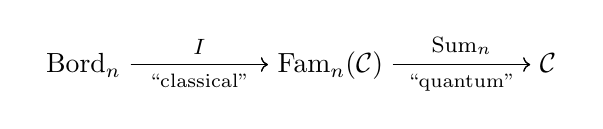
\begin{tikzpicture}[
			     baseline=(current bounding box.base), 
			     %>=stealth,
			     descr/.style={fill=white,inner sep=3.5pt}, 
			     normal line/.style={->}
			     ] 
\matrix (m) [matrix of math nodes, row sep=3.5em, column sep=5.0em, text height=1.5ex, text depth=0.1ex] {%
\Bord_n  &  \textrm{Fam}_n(\Ccal)  &  \Ccal 
\\
};
\path[font=\footnotesize] (m-1-1) edge[->] node[above] {$I$} (m-1-2);
\path[font=\scriptsize] (m-1-1) edge[->] node[below] {$\textrm{``classical''}$} (m-1-2);
\path[font=\footnotesize] (m-1-2) edge[->] node[above] {$\textrm{Sum}_n$} (m-1-3);
\path[font=\scriptsize] (m-1-2) edge[->] node[below] {$\textrm{``quantum''}$} (m-1-3);
\end{tikzpicture}
%%%%%%%%%%%%%%%%%%%%%%% 
\ee
based on the data $(G,\omega)$, which is viewed as a fully extended version of Dijkgraaf-Witten theory. 
On the other hand, in \cite{WittenParity2016, WWW} a class of boundary conditions for (classical!?) DW theory is proposed in terms of group extensions. 

\medskip

\noindent
\textbf{Goal. }
We want to reformulate the general aspects of the work \cite{WittenParity2016, WWW} in the setting of fully extended TQFT. 
More precisely, we view the bulk theories of \cite{WittenParity2016, WWW} as the classical part~$I$ in \eqref{eq:TQFTfactored} with $\Ccal = \boldB^n \C^\times$ (the $n$-fold delooping of the group~$\C^\times$) and then 
\begin{enumerate}
\item
identify \textsl{classical} boundary conditions as 1-morphisms with source $*$ in $\textrm{Fam}_n(\boldB^n \C^\times)$, 
\item
subsume the boundary conditions of \cite{WittenParity2016, WWW} as special cases, 
\item
map classical boundary conditions to quantum ones via $\textrm{Sum}_n$, and connect them to the known quantum boundary conditions, following the work of Ostrik and Fuchs--Schweigert--Valentino in the case $n=3$, 
\item 
do the above not only for framed, but also for oriented, spin,\dots TQFTs. 
\end{enumerate}

\medskip

Since \cite{FHLT} is very light on details, we first will work out explicitly how \eqref{eq:TQFTfactored} recovers the known bulk theory for $n \in \{1,2\}$ and hopefully also $n=3$. 
We also want to explain in detail how $(G,\omega)$ gives rise to an object in $\textrm{Fam}_n(\boldB^n \C^\times)$, and how group extensions $1 \to K \to H \stackrel{r}{\to} G \to 1$ give rise to 1-morphisms $\textrm{Fam}_n(\boldB^n \C^\times)(*, \boldB G)$. 
\\
(A more conceptual approach to boundary conditions and defects would be to start with a bordism category ``with singularities'' \cite[Sect.\,4.3]{l0905.0465} instead of $\Bord_n$, but we leave that for another project.)


\section{Special objects and 1-morphisms in $\textrm{Fam}_n(\boldB^n \C^\times)$}
\label{sec:FamBnC}

TODO: 
\begin{itemize}
\item 
spell out definition of $\textrm{Fam}_n(\Ccal)$
\item
check that $n$-functor $\boldB G \to \boldB^n \C^\times$ is precisely an $n$-cocycle
\\
\underline{\textbf{Issue}}: For $n>3$, what is a weak $n$-functor, i.\,e.~precisely what data and constraints are needed?
\\
\underline{\textbf{Idea}}: Since both $n$-categories in $\boldB G \to \boldB^n \C^\times$ are close to trivial, most data of the functor will be trivial, and the constraints (whatever they are) will be trivially satisfied. 
For $n \in \{1,2,3\}$ this is true, see Section~\ref{sec:bulk}. 
\item 
clarify precisely how $\boldB G \to \boldB^n \C^\times$ induces an $n$-functor $\boldB G \to n$-Vect, at least for $n \in \{1,2,3\}$
\item 
check whether natural transformation from trivial $n$-functor to $\omega \circ r$ is trivialisation of $r^* \omega$
\\
\underline{\textbf{Issue}}: induced from issue in second item
\end{itemize}


\section{Bulk theory}
\label{sec:bulk}

\subsection[$n=1$]{$\boldsymbol{n=1}$}

Since we take the action of~$G$ on~$\C^\times$ to be trivial, the cocycle 
\be
\omega = [\omega] \in H^1(G,\C^\times) = \Hom_{\text{Grp}}(G,\C^\times)
\ee
is just a group homomorphism. 
We consider $\boldB^1 \C^\times$ as a subcategory of $\Vect_\C$, and we will use the pair $(G,\omega)$ to construct a functor
\be
\label{eq:TQFTfactored1}
%%%%%%%%%%%%%%%%%%%%%%%
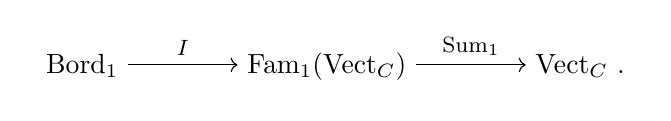
\begin{tikzpicture}[
			     baseline=(current bounding box.base), 
			     %>=stealth,
			     descr/.style={fill=white,inner sep=3.5pt}, 
			     normal line/.style={->}
			     ] 
\matrix (m) [matrix of math nodes, row sep=3.5em, column sep=4.0em, text height=1.5ex, text depth=0.1ex] {%
\Bord_1  &  \textrm{Fam}_1(\Vect_\C)  &  \Vect_\C \, . 
\\
};
\path[font=\footnotesize] (m-1-1) edge[->] node[above] {$I$} (m-1-2);
\path[font=\footnotesize] (m-1-2) edge[->] node[above] {$\textrm{Sum}_1$} (m-1-3);
\end{tikzpicture}
%%%%%%%%%%%%%%%%%%%%%%% 
\ee

According to the cobordism hypothesis, the composite $\textrm{Sum}_1 \circ I$ is determined by its value on the point $\text{pt}_+$, so we only need to specify $I(\text{pt}_+)$ and then compute $\textrm{Sum}_1(I(\text{pt}_+))$. 
Note that $\boldB^1 G = */\!\!/ G$ is the classical action groupoid. 
We set $I(\text{pt}_+)$ to be the functor
\be
\chi^\omega \colon */\!\!/ G \lra \Vect_\C 
\, , \qquad 
* \lmt \C
\, , \quad 
g \lmt \omega(g) \in \text{Aut}(\C)
\ee
%which sends~$*$ to~$\C$ and~$g$ to $\omega(g) \in \text{Aut}(\C)$ 
for all $g \in G$. 
Then \eqref{eq:TQFTfactored1} recovers the known result reviewed in \cite[Sect.\,1]{FHLT}: 

\begin{lemma}\label{lemma:cocone-is-coinvariants}
$\text{Sum}_1(\chi^\omega) = \C$ if $\omega(g) = 1$ for all $g\in G$, and $\text{Sum}_1(\chi^\omega) = 0$ otherwise. 
\end{lemma}

\begin{proof}
The statement is a particular case of this more general one: let $(V,\rho)$ be a linear representation of the group $G$, seen as the functor
\be
\chi^\rho \colon */\!\!/ G \lra \Vect_\C 
\, , \qquad 
* \lmt V
\, , \quad 
g \lmt \rho(g) \in \text{Aut}(V).
\ee
Then the universal cocone of $\chi^\rho$, viewed as a diagram of shape $*/\!\!/ G$ in $\Vect_\C$ is the pair $(V_G,\pi)$, where $V_G$ is the vector space of coinvariants for the representation $\rho$, i.e., 
\[
V_G=V/\langle v-\rho(g)v\rangle_{g\in G, v\in V}
\]
and $\pi\colon V\to V_G$ is the projection to the quotient. Namely, let $(W,f)$ be a cocone for $\chi^\rho$, i.e., a pair consisting of a vector space $W$ together with a linear map $f\colon \chi^\omega(*) = V \to W$ such that 
\be
%%%%%%%%%%%%%%%%%%%%%%%
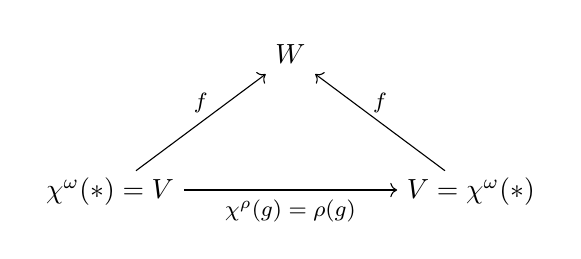
\begin{tikzpicture}[
			     baseline=(current bounding box.base), 
			     %>=stealth,
			     descr/.style={fill=white,inner sep=3.5pt}, 
			     normal line/.style={->}
			     ] 
\matrix (m) [matrix of math nodes, row sep=3.5em, column sep=3.0em, text height=1.5ex, text depth=0.1ex] {%
  &  W  &  
\\
\chi^\omega(*) = V &    &  V = \chi^\omega(*)
\\
};
\path[font=\footnotesize] (m-2-1) edge[->] node[above] {$f$} (m-1-2);
\path[font=\footnotesize] (m-2-1) edge[->] node[below] {$\chi^\rho(g) = \rho(g)$} (m-2-3);
\path[font=\footnotesize] (m-2-3) edge[->] node[above] {$f$} (m-1-2);
\end{tikzpicture}
%%%%%%%%%%%%%%%%%%%%%%% 
\ee
Then, by definition of $V_G$, the morphism $f$ uniquely factors through $V_G$ and so we have a commutative diagram
\be
%%%%%%%%%%%%%%%%%%%%%%%
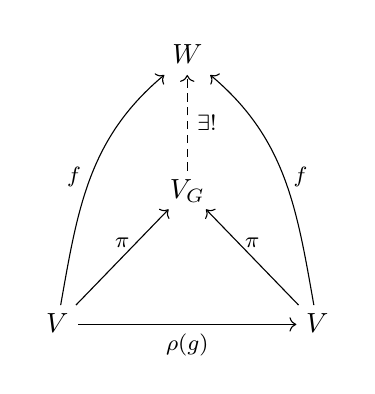
\begin{tikzpicture}[
			     baseline=(current bounding box.base), 
			     %>=stealth,
			     descr/.style={fill=white,inner sep=3.5pt}, 
			     normal line/.style={->}
			     ] 
\matrix (m) [matrix of math nodes, row sep=3.5em, column sep=3.0em, text height=1.5ex, text depth=0.1ex] {%
  &  W  &  
\\
  &  V_G  &  
\\
V  &    &  V
\\
};
\path[font=\footnotesize] (m-3-1) edge[->] node[above] {$\pi$} (m-2-2);
\path[font=\footnotesize] (m-3-1) edge[->] node[below] {$\rho(g)$} (m-3-3);
\path[font=\footnotesize] (m-3-3) edge[->] node[above] {$\pi$} (m-2-2);
%
\path[font=\footnotesize] (m-3-1) edge[->, out= 80, in= 220] node[left] {$f$} (m-1-2);
\path[font=\footnotesize] (m-3-3) edge[->, out= 100, in= -40] node[right] {$f$} (m-1-2);
%
\path[font=\footnotesize, densely dashed] (m-2-2) edge[->] node[right] {$\exists !$} (m-1-2);
\end{tikzpicture}
%%%%%%%%%%%%%%%%%%%%%%% 
\ee

%Hence $\text{Sum}_1(\chi^\omega)$ is in particular a cocone of $\chi^\omega$, i.\,e.~a vector space~$V$ together with a linear map $f\colon \chi^\omega(*) = \C \to V$ such that 
%\be
%%%%%%%%%%%%%%%%%%%%%%%%
%\begin{tikzpicture}[
%			     baseline=(current bounding box.base), 
%			     %>=stealth,
%			     descr/.style={fill=white,inner sep=3.5pt}, 
%			     normal line/.style={->}
%			     ] 
%\matrix (m) [matrix of math nodes, row sep=3.5em, column sep=3.0em, text height=1.5ex, text depth=0.1ex] {%
%  &  V  &  
%\\
%\chi^\omega(*) = \C  &    &  \C = \chi^\omega(*)
%\\
%};
%\path[font=\footnotesize] (m-2-1) edge[->] node[above] {$f$} (m-1-2);
%\path[font=\footnotesize] (m-2-1) edge[->] node[below] {$\chi^\omega(g) = \omega(g)$} (m-2-3);
%\path[font=\footnotesize] (m-2-3) edge[->] node[above] {$f$} (m-1-2);
%\end{tikzpicture}
%%%%%%%%%%%%%%%%%%%%%%%% 
%\ee
%commutes for all $g\in G$. 
%If $\omega(g) \neq 1$ for some~$g$, then this forces $f=0$, and the colimit is trivial: 
%\be
%%%%%%%%%%%%%%%%%%%%%%%%
%\begin{tikzpicture}[
%			     baseline=(current bounding box.base), 
%			     %>=stealth,
%			     descr/.style={fill=white,inner sep=3.5pt}, 
%			     normal line/.style={->}
%			     ] 
%\matrix (m) [matrix of math nodes, row sep=3.5em, column sep=3.0em, text height=1.5ex, text depth=0.1ex] {%
%  &  0  &  
%\\
%  &  V  &  
%\\
%\C  &    &  \C
%\\
%};
%\path[font=\footnotesize] (m-3-1) edge[->] node[above] {$f$} (m-2-2);
%\path[font=\footnotesize] (m-3-1) edge[->] node[below] {$\omega(g)$} (m-3-3);
%\path[font=\footnotesize] (m-3-3) edge[->] node[above] {$f$} (m-2-2);
%%
%\path[font=\footnotesize] (m-3-1) edge[->, out= 80, in= 220] node[left] {$0$} (m-1-2);
%\path[font=\footnotesize] (m-3-3) edge[->, out= 100, in= -40] node[right] {$0$} (m-1-2);
%%
%\path[font=\footnotesize, densely dashed] (m-2-2) edge[->] node[right] {$\exists !$} (m-1-2);
%\end{tikzpicture}
%%%%%%%%%%%%%%%%%%%%%%%% 
%\ee
%On the other hand, if~$\omega$ is trivial, every pair $(V,f)$ is a cocone, but the universal cocone is $(\C,1)$. 
showing that $(V_G,\pi)$ enjoys the universal property of the universal cocone.
\end{proof}

\begin{corollary}
The linear dual $\mathrm{Hom}_{\Vect_\C}(\text{Sum}_1(\chi^\omega),\C)$ of $\text{Sum}_1(\chi^\omega)$ is naturally isomorphic to the vector space of natural transformations $\mathrm{Hom}_{[*/\!\!/ G,\Vect_\C]}(\chi^\omega,\chi^1)$, where $\chi^1\colon  */\!\!/ G \to \Vect_\C$ is the trivial representation of $G$ on the vector space $\C$. In other words, we have
\[
\mathrm{Hom}_{\Vect_\C}(\text{Sum}_1(\chi^\omega),\C)\cong \left\{
\raisebox{40pt}{\xymatrix{
{*}/\!\!/ G\ar[dd]_{\chi^\omega}\ar[dr]\\
&{*}\ar[dl]^{\C}\\
\Vect_\C
\ar@{=>}(5,-13);(10,-13)
}}
\right\}.
\]
As a finite dimensional vector space is completely determined by its linear dual, this actually defines $\text{Sum}_1(\chi^\omega)$.
\end{corollary}
\begin{proof}
Again, the statement is true for an aritrary linear representation $(V,\rho)$ of the group $G$. The natural isomorphism
\[
\mathrm{Hom}_{\Vect_\C}(V_G,\C)\cong \left\{
\raisebox{40pt}{\xymatrix{
{*}/\!\!/ G\ar[dd]_{\chi^\rho}\ar[dr]\\
&{*}\ar[dl]^{\C}\\
\Vect_\C
\ar@{=>}(5,-13);(10,-13)
}}
\right\}
\]
is then nothing but the universal property of $V_G$. Namely, an element in the right hand side is a morphism $f\colon V=\chi^\rho(*)\to \chi^1(*)=\C$ such that all the diagrams
\[
\xymatrix{
V\ar[d]_{\rho(g)}\ar[r]^f & \C\ar[d]^{\mathrm{id}_\C}\\
V\ar[r]_f &\C
}
\]
commute, for any $g\in G$. This is the same as requiring that all the diagrams
\[
\xymatrix{
&\C\\
V\ar[rr]_{\rho(g)}\ar[ru]^{f} &&V\ar[lu]_{f}
}
\]
commute, and so it is precisely the datum of a morphism $V_G\to \C$ by the argumenti in the proof of Lemma \ref{lemma:cocone-is-coinvariants}.
\end{proof}


\subsection[$n=2$]{$\boldsymbol{n=2}$}

\subsubsection{``Without thinking'' (Nils)}

Now let $\omega \in Z^2(G,\C^\times)$. 
We will construct a 2-functor 
\be
\label{eq:TQFTfactored2}
%%%%%%%%%%%%%%%%%%%%%%%
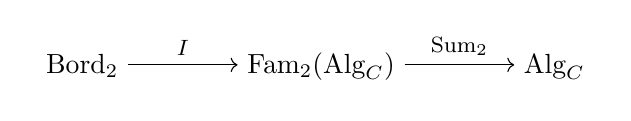
\begin{tikzpicture}[
			     baseline=(current bounding box.base), 
			     %>=stealth,
			     descr/.style={fill=white,inner sep=3.5pt}, 
			     normal line/.style={->}
			     ] 
\matrix (m) [matrix of math nodes, row sep=3.5em, column sep=4.0em, text height=1.5ex, text depth=0.1ex] {%
\Bord_2  &  \textrm{Fam}_2(\text{Alg}_\C)  &  \text{Alg}_\C 
\\
};
\path[font=\footnotesize] (m-1-1) edge[->] node[above] {$I$} (m-1-2);
\path[font=\footnotesize] (m-1-2) edge[->] node[above] {$\textrm{Sum}_2$} (m-1-3);
\end{tikzpicture}
%%%%%%%%%%%%%%%%%%%%%%% 
\ee
by computing what it does to $\text{pt}_+ \in \Bord_2$. 
The first step is to set $I(\text{pt}_+)$ to be the 2-functor 
\begin{align}
\chi^\omega \colon \boldB G 
& \lra \Algc 
&& \text{with} \quad \chi^\omega_{g,h} := \omega(g,h) \colon L_g \otimes_\C L_h \to L_{gh}
\label{eq:chiomega2}
\\
* & \lmt \C && \nonumber
\\
G \ni g & \lmt L_g := {}_\C \C_\C && \nonumber && \nonumber
\\
1_g & \lmt  1_\C && \nonumber
\end{align}
(Recall from \cite[Sect.\,1.1]{LeinsterBasic2} that the constraint on the coherence 2-morphisms $\chi^\omega_{g,h} = \omega(g,h) \in \End_\C(\C)$ is precisely the 2-cocycle condition on~$\omega$. 
Also note that all our 2-functors are strictly unital, so in particular~\eqref{eq:chiomega2} completely specifies the 2-functor~$\chi^\omega$.) 

The second step is to compute the 2-colimit $\text{Sum}_2(\chiom)$. 
There are several versions of 2-limit, bilimit, weighted bilimit etc.~in the literature.  
We will use the notion of \cite[Def.\,7.4.4]{bor94} and call it 2-limit. 
To give the details, recall the definitions from \cite[Sect.\,1.2--3]{LeinsterBasic2}, and that the \textsl{opposite} $\B^{\text{op}}$ of a bicategory~$\B$ has reversed horizontal composition, but the same vertical composition as~$\B$. 

\begin{definition}
\label{def:2limit}
Let $F \colon \mathcal A \to \B$ be a 2-functor, and let $B\in\B$. 
\begin{enumerate}
\item
The \textsl{constant 2-functor} $\Delta_B \colon \mathcal A \to \B$ sends every object in~$\mathcal A$ to~$B$, 1- and 2-morphisms in~$\mathcal A$ to $1_B$ and $1_{1_B}$, respectively, and all constraints $(\Delta_B)_{g,h}$ are trivial. 
\item 
The category $2\text{-Cone}(B,F)$ of \textsl{2-cones on~$F$ with vertex~$B$} is the category whose objects are pseudonatural transformations $\Delta_B \to F$ and whose morphisms are modifications between them. 
\item 
A \textsl{2-limit} of~$F$ is a pair $(L,\pi)$ with $B\in \B$ and $\pi \colon \Delta_L \to F$ a pseudonatural transformation such that the functor
\begin{align*}
%\pi_* \colon 
\B(B,L) 
& \lra 2\text{-Cone}(B,F) 
\\
(B \stackrel{f}{\lra} L) 
& \lmt (\Delta_B \stackrel{f_*}{\lra} \Delta_L \stackrel{\pi}{\lra} F) 
\end{align*}
is an equivalence of categories for all $B\in\B$. 
\item 
Now let $G \colon \mathcal A \to \B^{\text{op}}$. 
The category $2\text{-Cocone}(B,G)$ of \textsl{2-cocones on~$G$ with vertex $B \in \B$} is defined to be $2\text{-Cone}(B,G)$, but with~$B$ viewed as an object in $\B^{\text{op}}$. 
A 2-limit of $G \colon \mathcal A \to \B^{\text{op}}$ is also called a \textsl{2-colimit of~$G$ in~$\B$}. 
\end{enumerate}
\end{definition}

Spelling out the definition, we see that an object $\sigma \colon \Delta_B \to F$ of $2\text{-Cone}(B,F)$ is a family of 1- and 2-morphisms 
\be
\label{eq:2cone1}
\big\{ B \stackrel{\sigma_A}{\lra} F(A) \big\}_{A\in\mathcal A}
\quad\text{ and }\quad 
\big\{ F(g) \otimes \sigma_A \stackrel{\sigma_g}{\lra} \sigma_{A'} \big\}_{g\in\mathcal A(A,A')}
\ee
such that 
\be
\label{eq:2cone2}
%%%%%%%%%%%%%%%%%%%%%%%
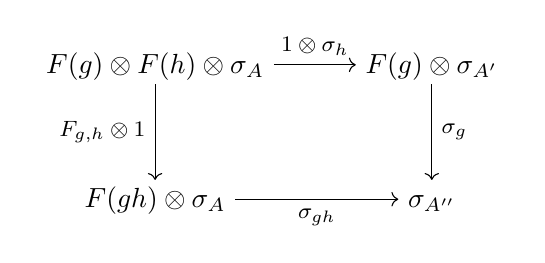
\begin{tikzpicture}[
			     baseline=(current bounding box.base), 
			     %>=stealth,
			     descr/.style={fill=white,inner sep=3.5pt}, 
			     normal line/.style={->}
			     ] 
\matrix (m) [matrix of math nodes, row sep=3.5em, column sep=3.0em, text height=1.5ex, text depth=0.1ex] {%
F(g) \otimes F(h) \otimes \sigma_A  &  F(g) \otimes \sigma_{A'}
\\
F(gh) \otimes \sigma_A  & \sigma_{A''}
\\
};
\path[font=\footnotesize] (m-1-1) edge[->] node[above] {$1\otimes \sigma_h$} (m-1-2);
\path[font=\footnotesize] (m-1-1) edge[->] node[left] {$F_{g,h} \otimes 1$} (m-2-1);
\path[font=\footnotesize] (m-2-1) edge[->] node[below] {$\sigma_{gh}$} (m-2-2);
\path[font=\footnotesize] (m-1-2) edge[->] node[right] {$\sigma_{g}$} (m-2-2);
\end{tikzpicture}
%%%%%%%%%%%%%%%%%%%%%%% 
\ee
commutes for all 
$
A \stackrel{h}{\lra} A' \stackrel{g}{\lra} A''
$. 
Furthermore, a morphism $\Gamma \colon \sigma \to \widetilde\sigma$ in $2\text{-Cone}(B,F)$ is a family 
\be
\label{eq:2cone3}
\big\{ \sigma_A \stackrel{\Gamma_A}{\lra} \widetilde\sigma_A \big\}_{A\in\mathcal A}
\quad\text{ such that }\quad 
%%%%%%%%%%%%%%%%%%%%%%%
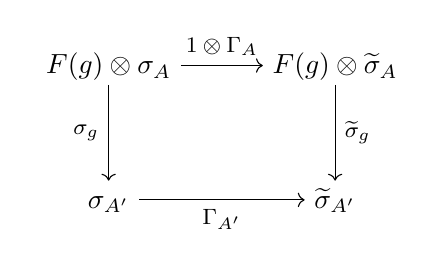
\begin{tikzpicture}[
			     baseline=(current bounding box.base), 
			     %>=stealth,
			     descr/.style={fill=white,inner sep=3.5pt}, 
			     normal line/.style={->}
			     ] 
\matrix (m) [matrix of math nodes, row sep=3.5em, column sep=3.0em, text height=1.5ex, text depth=0.1ex] {%
F(g) \otimes \sigma_A  &  F(g) \otimes \widetilde\sigma_A
\\
\sigma_{A'}  & \widetilde\sigma_{A'}
\\
};
\path[font=\footnotesize] (m-1-1) edge[->] node[above] {$1\otimes \Gamma_A$} (m-1-2);
\path[font=\footnotesize] (m-1-1) edge[->] node[left] {$\sigma_g$} (m-2-1);
\path[font=\footnotesize] (m-2-1) edge[->] node[below] {$\Gamma_{A'}$} (m-2-2);
\path[font=\footnotesize] (m-1-2) edge[->] node[right] {$\widetilde\sigma_{g}$} (m-2-2);
\end{tikzpicture}
%%%%%%%%%%%%%%%%%%%%%%% 
\ee
commutes for all 
$
A \stackrel{g}{\lra} A'
$. 

Note that above ``$\otimes$'' is exclusively used for the horizontal composition in the target~$\B$ (while juxtaposition is used for the horizontal composition in~$\mathcal A$). 
Hence going to $\B^{\text{op}}$ amounts to reversing all the tensor products above. 

\begin{lemma}
\label{lem:2cone}
Let $B\in \Algc$ and $\chiom \colon \boldB G \to \Algc$ as in~\eqref{eq:chiomega2}. 
Then 
\begin{align}
2\text{-Cone}(B,\chiom) & \cong  {}_{\CGtw}\text{Mod}_B \, , \nonumber 
\\
2\text{-Cocone}(B,\chiom) & \cong  {}_{B}\text{Mod}_{\CGtw}
\end{align}
where $\CGtw$ is the $\omega$-twisted group algebra of~$G$. 
\end{lemma}

\begin{proof}
We only prove the the statement about 2-cones in detail, the one about 2-cocones follows analogously by reversing all horizontal compositions in~$\B$. 

By \eqref{eq:2cone1} and \eqref{eq:2cone2}, an object in $2\text{-Cone}(B,\chiom)$ is a 1-morphism $M \in \Algc(B,\C)$ together with linear maps $\sigma_g \colon L_g \otimes_\C M \to M$ such that 
\be
%%%%%%%%%%%%%%%%%%%%%%%
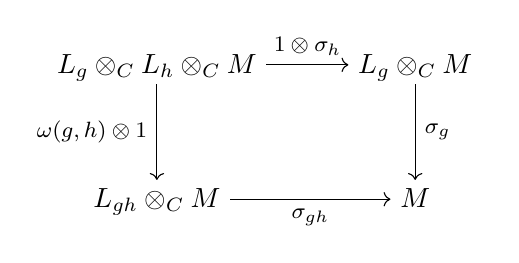
\begin{tikzpicture}[
			     baseline=(current bounding box.base), 
			     %>=stealth,
			     descr/.style={fill=white,inner sep=3.5pt}, 
			     normal line/.style={->}
			     ] 
\matrix (m) [matrix of math nodes, row sep=3.5em, column sep=3.0em, text height=1.5ex, text depth=0.1ex] {%
L_g \otimes_\C L_h \otimes_\C M  &  L_g \otimes_\C M
\\
L_{gh} \otimes_\C M  & M
\\
};
\path[font=\footnotesize] (m-1-1) edge[->] node[above] {$1\otimes \sigma_h$} (m-1-2);
\path[font=\footnotesize] (m-1-1) edge[->] node[left] {$\omega(g,h) \otimes 1$} (m-2-1);
\path[font=\footnotesize] (m-2-1) edge[->] node[below] {$\sigma_{gh}$} (m-2-2);
\path[font=\footnotesize] (m-1-2) edge[->] node[right] {$\sigma_{g}$} (m-2-2);
\end{tikzpicture}
%%%%%%%%%%%%%%%%%%%%%%% 
\ee
commutes for all $g,h \in G$. 
But this means that $(M, \sum_{g\in G} \sigma_g$) is a left $\CGtw$-module, while by definition of $\Algc$, the 1-morphism $M \in \Algc(B,\C)$ is a right $B$-module. 

According to \eqref{eq:2cone3}, a morphism $(M, \{ \sigma_g \}) \to (\widetilde M, \{ \widetilde\sigma_g \})$ in $2\text{-Cone}(B,\chiom)$ is a 2-morphism $\Gamma \colon {}_\C M_B \to {}_\C \widetilde M_B$ in $\Algc$ such that 
\be
%%%%%%%%%%%%%%%%%%%%%%%
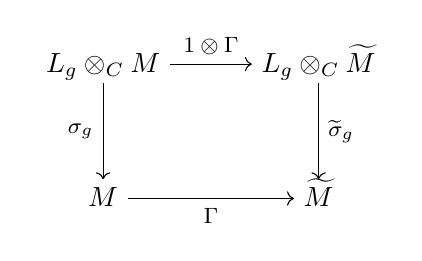
\begin{tikzpicture}[
			     baseline=(current bounding box.base), 
			     %>=stealth,
			     descr/.style={fill=white,inner sep=3.5pt}, 
			     normal line/.style={->}
			     ] 
\matrix (m) [matrix of math nodes, row sep=3.5em, column sep=3.0em, text height=1.5ex, text depth=0.1ex] {%
L_g \otimes_\C M  &  L_g \otimes_\C \widetilde M
\\
M  & \widetilde M
\\
};
\path[font=\footnotesize] (m-1-1) edge[->] node[above] {$1\otimes \Gamma$} (m-1-2);
\path[font=\footnotesize] (m-1-1) edge[->] node[left] {$\sigma_g$} (m-2-1);
\path[font=\footnotesize] (m-2-1) edge[->] node[below] {$\Gamma$} (m-2-2);
\path[font=\footnotesize] (m-1-2) edge[->] node[right] {$\widetilde\sigma_{g}$} (m-2-2);
\end{tikzpicture}
%%%%%%%%%%%%%%%%%%%%%%% 
\ee 
commutes. 
But that means that~$\Gamma$ is both a map of left $\CGtw$-modules and a map of right $B$-modules. 
\end{proof}

\begin{proposition}
\begin{enumerate}
\item
A 2-limit of $\chiom \colon \boldB G \to \Algc$ is given by $(\CGtw, \CGtw)$. 
\item
A 2-colimit of $\chiom \colon \boldB G \to \Algc$ is given by $(\CGtw, \CGtw)$. 
\end{enumerate}
\end{proposition}

\begin{proof}
According to Definition~\ref{def:2limit} and Lemma~\ref{lem:2cone}, a 2-limit of $\chiom$ is an algebra $L \in \Algc$ together with a module ${}_{\CGtw} M_L$ such that the functor 
\begin{align*}
\Algc(B,L) 
& \lra {}_{\CGtw}\text{Mod}_B
\\
N & \lmt M \otimes_L N
\end{align*}
is an equivalence for every $B \in \Algc$. 
This is the case for $L = \CGtw$ as an algebra and $M = \CGtw$ as a bimodule over itself. 

The statement about the 2-colimit follows analogously. 
\end{proof}


\subsubsection{``With thinking'' (Domenico)}

The datum of the 2-functor $\chi^\omega \colon \boldB G \to \text{Alg}_\C$ is a collection of lines (1-dimensional complex vector spaces) $L_g$, indexed by elements in the group $G$, together with isomorphisms
\[
\rho_{g,h}\colon L_g\otimes L_h\xrightarrow{\sim} L_{gh}
\]
subject to the associativity constraint given by the commutativity of the diagrams
\[
\xymatrix{
L_g\otimes L_h\otimes L_k\ar[rr]^{\rho_{g,h}\otimes \mathrm{id}}\ar[d]_{\mathrm{id}\otimes \rho_{h,k}}&& L_{gh}\otimes L_k\ar[d]^{\rho_{gh,k}}\\
L_g\otimes L_{hk}\ar[rr]_{\rho_{g,hk}} &&L_{ghk}
}
\]
where the tensor products are over $\C$. We also require that $L_1=\C$ and that the isomorphisms $L_1\otimes L_g\xrightarrow{\sim}L_g$ and $L_g\otimes L_1\xrightarrow{\sim}L_g$ are the structure isomorphisms for the unit object $\C$ of the monoidal category $\mathrm{Vect}_\C$.
The associativity constraints imply, and are in fact equivalent to this, that the vector space
\[
A_{\chi^\omega}=\bigoplus_{g\in G} L_g
\]
has an associative $\C$-algebra structure.
\begin{lemma}
A choice of a basis element $x_g$ for every line $L_g$ defines a $\C^\times$-valued 2-cocycle $\omega$ on the group $G$. A different choice of basis elements leads to a cohomologous cocycle, so that the class $[\omega]\in H^2(G,\C^\times)$ is well defines.
\end{lemma}
\begin{proof}
As $\rho_{g,h}(x_g\otimes x_h)$ is a nonzero element in $L_{gh}$ we have $\rho_{g,h}(x_g\otimes x_h)=\omega(g,h)x_{gh}$ for a unique element $\omega(g,h)$ in $\C^\times$. The associativity constraints are then immediately seen to be equivalent to the cocycle equation
\[
\omega(gh,k)\omega(g,h)=\omega(g,hk)\omega(h,k).
\]
Finally, if $\{y_g\}_{g\in G}$ is a different basis choice, and $\tilde{\omega}$ is the corresponding 2-cocycle, then we have $y_g=\eta_gx_g$ for some $\eta_g$ in $\C^\times$ and
\[
\tilde{\omega(g,h)}y_{gh}=\rho_{g,h}(y_g\otimes y_h)=\eta_g\eta_h\rho_{g,h}(x_g\otimes x_h)=\eta_g\eta_h\omega(g,h)x_{gh}=\eta_g\eta_h\omega(g,h)\eta_{gh}^{-1}y_{gh}.
\]
Therefore
\[
\tilde{\omega}(g,h)=\eta_g\eta_{gh}^{-1}\eta_h\omega(g,h),
\]
i.e. $\omega$ and $\tilde{\omega}$ are cohomologous.
\end{proof}
\begin{corollary}
The algebra $A_{\chi^\omega}$ is isomorphic to the twisted group algebra $\C^\omega[G]$, defined as the $\C$-vector space on the basis $\{x_g\}_{g\in G}$ with the product $x_g\cdot x_h=\omega(g,h)x_{gh}$ and with $x_1=1$.
\end{corollary}
\begin{lemma}\label{lemma:cocone-is-coinvariants}
$\text{Sum}_2(\chi^\omega) \cong \C^\omega[G]$, the  twisted group algebra of $G$.
\end{lemma}

\begin{proof}
Let $(A,M)$ be a cocone for $\chi^\omega$, i.e., a pair consisting of a $\C$-algebra $A$ together with a left $A$-module $M$ (representing a linear functor ${}_\C\mathrm{Mod}\to {}_A\mathrm{Mod}$) and homotopy commutative diagrams
\[
\xymatrix{
&A\\
\C\ar[rr]_{L_g}\ar[ur]^{M}&&\C\ar[lu]_M
\ar@{=>}^{\lambda_g}(18,-11);(9,-6)}
\]
where the $\lambda_g$'s are isomorphisms of left $A$-modules
\[
\lambda_g\colon  M\otimes_\C L_g\xrightarrow{\sim} M
\]
such that the diagrams
\[
\xymatrix{
M\otimes L_g\otimes L_h\ar[rr]^{\lambda_{g}\otimes \mathrm{id}}\ar[d]_{\mathrm{id}\otimes \rho_{g,h}}&& M\otimes L_h\ar[d]^{\lambda_h}\\
M\otimes L_{gh}\ar[rr]_{\lambda_{gh}} &&M
}
\]
commute. This implies that the isomorphisms $\lambda_g$ make $M$ a right $A_{\chi^\omega}$-module. Therefore, we can see $M$ as a linear functor 
\[
{}_{A_{\chi^\omega}}\mathrm{Mod}\to {}_A\mathrm{Mod}
\]
i.e., as a morphism from $A_{\chi^\omega}$ to $A$ in $2\text{-}\mathrm{Vect}_\C$. The algebra $A_{\chi^\omega}$ seen as a left $A_{\chi^\omega}$-module is a morphism from $\C$ to $A_{\chi^\omega}$ in $2\text{-}\mathrm{Vect}_\C$ and the natural isomorphism
\[
{}_AM_\C\cong {}_AM_{A_{\chi^\omega}}\otimes {}_{A_{\chi^\omega}}{A_{\chi^\omega}}_\C
\]
gives a canonical factorization
\[
\xymatrix{
&A\\
&A_{\chi^\omega}\ar[u]^{M}\\
\C\ar[rr]_{L_g}\ar[ur]^{A_{\chi^\omega}}\ar@/^2pc/[ruu]^{M}&&\C\ar[lu]_{A_{\chi^\omega}}\ar@/_2pc/[luu]_{M}
\ar@{=>}^{\lambda_g}(15,-26);(22,-21)}
\]
exhibiting the algebra $A_{\chi^\omega}$ together with itself seen as a left module over itself as the universal cocone. 
\end{proof}


\subsection[$n=3$]{$\boldsymbol{n=3}$}

TODO:
\begin{itemize}
\item
The only non-trivial part of the 3-functor $\chi^\omega \colon \boldB G \to \text{TC}_\C$ are the coherence 3-morphisms which assemble into the modification (also) called~$\omega$ in \cite[Def.\,A.4.3]{GregorDiss}, and the constraints on $\omega$ (see \cite[Page~219]{GregorDiss}) seem to be precisely the 3-cocycle condition. 
\item
\underline{\textbf{Issue}}: The notion of a 3-colimit (to really compute $\text{Sum}_3$) is scary. 
At least we should make some hand-wavy arguments\dots
\end{itemize}


\section{Boundary conditions}

\subsection[$n=2$]{$\boldsymbol{n=2}$}

TODO

\subsection[$n=3$]{$\boldsymbol{n=3}$}

TODO






\begin{thebibliography}{BDSPV}

\bibitem[Bo]{bor94}
F.~Borceux, 
\textsl{Handbook of categorical algebra 1}, 
volume 50 of \textsl{Encyclopedia of Mathematics and its Applications}, 
Cambridge University Press, Cambridge, 1994.

\bibitem[FHLT]{FHLT}
D.~Freed, M.~Hopkins, J.~Lurie, and C.~Teleman,
\textsl{Topological Quantum Field Theories from Compact Lie Groups}, 
\href{http://arxiv.org/abs/0905.0731}{[\mbox{arXiv:}0905.0731]}. 

\bibitem[Le]{LeinsterBasic2}
T.~Leinster, 
\textsl{Basic Bicategories}, 
\href{http://arxiv.org/abs/math/9810017}{[math/9810017]}.

\bibitem[Lu]{l0905.0465}
J.~Lurie, 
\textsl{On the Classification of Topological Field Theories},
\href{https://projecteuclid.org/euclid.cdm/1254748657}{Current Developments in Mathematics \textbf{2008} (2009), 129--280}, 
\arxiv{0905.0465}{[arXiv:0905.0465]}.

\bibitem[Sc]{GregorDiss}
G.~Schaumann, 
\textsl{Duals in tricategories and in the tricategory of bimodule categories}, 
PhD thesis, 
Friedrich-Alexander-Universit\"at Erlangen-N\"urnberg (2013), 
% \url{http://opus4.kobv.de/opus4-fau/frontdoor/index/index/docId/3732}.
%\newline
%\href{http://opus4.kobv.de/opus4-fau/frontdoor/index/index/docId/3732}{http://opus4.kobv.de/opus4-fau/frontdoor/index/index/docId/3732}.
\href{http://nbn-resolving.de/urn/resolver.pl?urn:nbn:de:bvb:29-opus4-37321}{urn:nbn:de:bvb:29-opus4-37321}.

\bibitem[Wi]{WittenParity2016}
E.~Witten, 
\textsl{The ``Parity'' Anomaly On An Unorientable Manifold}, 
\href{http://arxiv.org/abs/1605.02391}{[arXiv:1605.02391]}.  

\bibitem[WWW]{WWW}
J.~Wang, X.-G.~Wen and E.~Witten, 
\textsl{Symmetric Gapped Interfaces of SPT and SET States: Systematic Constructions}, 
\href{http://arxiv.org/abs/1705.06728}{[arXiv:1705.06728]}.  




\end{thebibliography}



\end{document}

